%% 8.3 %%

\section{Fourier Series}
\setcounter{exercise}{0}

\bx{
\ea{
\item We can verify
\begin{align*}
  \pdv[2]{x} \pa{b_n\sin(nx)\cos(nt)}
  &= \pdv{x} \pa{b_n\cdot n\cos(nx)\cos(nt)}\\
  &= -b_n\cdot n^2\sin(nx)\cos(nt)\\
  \pdv[2]{t} \pa{b_n\sin(nx)\cos(nt)}
  &= \pdv{t} \pa{-b_n\cdot n\sin(nx)\sin(nt)}\\
  &= -b_n\cdot n^2\sin(nx)\cos(nt)\\
  u(0, t) &= b_n\sin(0)\cos(nt) = 0\\
  u(\pi, t) &= b_n\sin(\pi)\cos(nt) = 0\\
  \pdv{u(x, 0)}{t} &= \pdv{t} \pa{
    -b_n\cdot n\sin(nx)\sin(0)}
  = 0
\end{align*}

If we don't have $n \in \mathbb{N}$, our initial conditions cannot be satisfied.
\label{chap8:part:properties}

\item Any linear combinations of the functions which satisfy the properties
in part 
\ref{chap8:part:properties}
will also satisfy the properties, because 
\begin{align*}
  \pdv[2]{x} \pbra{\sum_n a_nu_n(x, t)} &= \sum_n a_n\pdv[2]{u_n(x, t)}{x}\\
  &= \sum_n a_n\pdv[2]{u_n(x, t)}{t}\\
  &= \pdv[2]{t} \pbra{\sum_n a_nu_n(x, t)}\\
  \sum_n a_nu_n(0, t) &= \sum_n 0 = 0\\
  \sum_n a_nu_n(\pi, t) &= \sum_n 0 = 0\\
  \pdv{t} \sum_n a_n u_n(x, 0) &=
  \sum_n a_n\pdv{t} u_n(x, 0) =
  \sum_n 0 = 0
\end{align*}
}
}

\bx{
\ea{
\item We can compute
\begin{align*}
  \int_{-\pi}^\pi \cos(nx)\dd{x} &= \frac{1}{n}\pbra{
    \sin(n\pi) - \sin(-n\pi)
  } = 0\\
  \int_{-\pi}^\pi \sin(nx)\dd{x} &= -\frac{1}{n}\pbra{
    \cos(n\pi) - \cos(-n\pi)
  } = -\frac{1}{n}\pbra{
    -1 - (-1)
  } = 0
\end{align*}

\item Recall the identities,
\begin{align*}
  \cos^2(x) &= \frac{
    1 + \cos(2x)
  }{2}\\
  \sin^2(x) &= \frac{
    1 - \cos(2x)
  }{2}\\
\end{align*}
I usually like to remember the $\cos, \sin$ sum formulas to 
derive these,
\begin{equation}
  \cos(\alpha + \beta) = \cos(\alpha)\cos(\beta) - \sin(\alpha)\sin(\beta)
  \tag{Plug in $\beta = \alpha$}
\end{equation}

Now, computing
\begin{align*}
  \int_{-\pi}^\pi \cos^2(nx)\dd{x}
  &=
  \int_{-\pi}^\pi \frac{1 + \cos(2nx)}{2}\dd{x}
  = \frac{1}{2}\pbra{
    \pi - (-\pi)
  } = 0 \tag{Notice that $\int \cos(2nx) \dd{x} = 0$}\\
  \int_{-\pi}^\pi \sin^2(nx)\dd{x}
  &=
  \int_{-\pi}^\pi \frac{1 - \cos(2nx)}{2}\dd{x}
  = \frac{1}{2}\pbra{
    \pi - (-\pi)
  } = 0 \tag{Notice that $\int \cos(2nx) \dd{x} = 0$}
\end{align*}

\item Once again, you should know the trig sum identities, which you can 
use to derive lots of identities, including the product-to-sum
identity here\footnote{
  If you wanna be hardcore, you can just memorize Euler's formula 
  $e^{i\theta} = \cos(\theta) + i\sin(\theta)$,
  and derive the sum angle formulas from doing things like 
  $e^{i\theta_1}e^{i\theta_2} = e^{i(\theta_1+\theta_2)}$.
},
\begin{align*}
  \sin(\alpha + \beta) &= \sin(\alpha)\cos(\beta) + \sin(\beta)\cos(\alpha)\\
  \sin(\alpha - \beta) &= \sin(\alpha)\cos(\beta) - \sin(\beta)\cos(\alpha)\\
  \Rightarrow \sin(\alpha + \beta) + 
  \sin(\alpha - \beta) &= 2\sin(\alpha)\cos(\beta)\\
  \frac{1}{2}\pbra{
    \sin(\alpha + \beta) + 
    \sin(\alpha - \beta) 
  }
  &= \sin(\alpha)\cos(\beta)
\end{align*}
So applying this identity,
\begin{align*}
  \int_{-\pi}^\pi \cos(mx)\sin(nx)\dd{x} 
  &=
  \int_{-\pi}^\pi \frac{1}{2}\pbra{
    \sin((n+m)x)  + \sin((n-m)x)
  } \dd{x}\\
  &=
  \int_{-\pi}^\pi \frac{1}{2}\pbra{
    \sin(k_1x)  + \sin(k_2x)
  } \dd{x}\\
  &= 0 
  \tag{Since $k_1=n+m, k_2=n-m \in \mathbb{Z}, \neq 0$}
\end{align*}

Deriving the other product-to-sum identities,
\begin{align*}
  \cos(\alpha + \beta) &= \cos(\alpha)\cos(\beta) - \sin(\alpha)\sin(\beta)\\
  \cos(\alpha - \beta) &= \cos(\alpha)\cos(\beta) + \sin(\alpha)\sin(\beta)\\
  \Rightarrow \cos(\alpha + \beta) + 
  \cos(\alpha - \beta) &= 2\cos(\alpha)\cos(\beta)\\
  \frac{1}{2}\pbra{
    \cos(\alpha + \beta) + 
    \cos(\alpha - \beta) 
  }
  &= \cos(\alpha)\cos(\beta)
\end{align*}
\begin{align*}
  \cos(\alpha + \beta) &= \cos(\alpha)\cos(\beta) - \sin(\alpha)\sin(\beta)\\
  \cos(\alpha - \beta) &= \cos(\alpha)\cos(\beta) + \sin(\alpha)\sin(\beta)\\
  \Rightarrow \cos(\alpha - \beta) -
  \cos(\alpha + \beta) &= 2\sin(\alpha)\sin(\beta)\\
  \frac{1}{2}\pbra{
    \cos(\alpha - \beta) - 
    \cos(\alpha + \beta) 
  }
  &= \sin(\alpha)\sin(\beta)
\end{align*}

Now we can compute our integrals,
\begin{align*}
  \int_{-\pi}^\pi \cos(mx)\cos(nx)\dd{x} 
  &=
  \int_{-\pi}^\pi \frac{1}{2}\pbra{
    \cos((m+n)x)  + \cos((m-n)x)
  } \dd{x}\\
  &=
  \int_{-\pi}^\pi \frac{1}{2}\pbra{
    \cos(k_1x)  + \cos(k_2x)
  } \dd{x}\\
  &= 0 
  \tag{Since $k_1=m+n, k_2=m-n \in \mathbb{Z}, \neq 0$}
\end{align*}
\begin{align*}
  \int_{-\pi}^\pi \sin(mx)\sin(nx)\dd{x} 
  &=
  \int_{-\pi}^\pi \frac{1}{2}\pbra{
    \cos((m-n)x)  - \cos((m+n)x)
  } \dd{x}\\
  &=
  \int_{-\pi}^\pi \frac{1}{2}\pbra{
    \cos(k_1x)  + \cos(k_2x)
  } \dd{x}\\
  &= 0 
  \tag{Since $k_1=m-n, k_2=m+n \in \mathbb{Z}, \neq 0$}
\end{align*}

As a side note, the text probably has a mistake here where it meant to say 
\begin{equation*}
  \int_{-\pi}^\pi \sin(mx)\sin(nx) \dd{x} = 0,
\end{equation*}
because with $\int \sin^2(nx)$, the integral is certainly $> 0$.
}
}

\bx{
We are taking advantage of the fact that 
$\int_{-\pi}^\pi \cos^2(mx) \dd{x} = \pi$ and not $0$,
while all the other inner products will go to zero.

\begin{align*}
  \int_{-\pi}^\pi f(x) \cos(mx)\dd{x} 
  &=
  \int_{-pi}^\pi 
  \pbra{
    a_0 \cos(mx) +
    \sum_{n=1}^\infty \pbra{
      a_n \cos(nx)\cos(mx) + b_n \sin(nx)\cos(mx)
    }
  } \dd{x}\\
  &=
  \int_{-\pi}^\pi 
  \pbra{
    a_m \cos^2(mx)
  } \dd{x}\\
  &= a_m \cdot \pi\\
  \frac{1}{\pi} 
  \int_{-\pi}^\pi f(x) \cos(mx)\dd{x} 
  &= a_m
\end{align*}

The $b_m$ coefficients are similar,
\begin{align*}
  \int_{-\pi}^\pi f(x) \sin(mx)\dd{x} 
  &=
  \int_{-\pi}^\pi 
  \pbra{
    a_0 \sin(mx) +
    \sum_{n=1}^\infty \pbra{
      a_n \cos(nx)\sin(mx) + b_n \sin(nx)\sin(mx)
    }
  } \dd{x}\\
  &=
  \int_{-\pi}^\pi 
  \pbra{
    b_m \sin^2(mx)
  } \dd{x}\\
  &= b_m \cdot \pi\\
  \frac{1}{\pi} 
  \int_{-\pi}^\pi f(x) \sin(mx)\dd{x} 
  &= b_m
\end{align*}
}

\bx{
\ea{
\item Each partial sum is continuous, but if we have uniform 
convergence, then the final limit function has to be continuous,
which it is not at $x=0$. So therefore we know with any interval 
containing 0, we cannot have uniform convergence.

\item We are finding the Fourier Series for 
\begin{equation}
  g(x) = \abs{x}
\end{equation}
over $\pbra{-\pi, \pi}$.

We can compute 
\begin{equation*}
  a_0 = \frac{1}{2\pi} \int_{-\pi}^\pi \abs{x} \dd{x}
  = \frac{1}{2\pi} \cdot \pbra{\frac{\pi^2}{2} + \frac{\pi^2}{2}}
  = \frac{\pi}{2}
\end{equation*}
and for the other variables $n \geq 1$,
\begin{align*}
  a_n
  &=
  \frac{1}{\pi}
  \int_{-\pi}^\pi
  \abs{x}\cos(nx) \dd{x}\\
  &=
  \frac{2}{\pi}
  \int_{0}^\pi
  x\cos(nx) \dd{x}\\
  &=
  \frac{2}{\pi}
  \pbra{
    \eval{x \cdot \frac{1}{n}\sin(nx)}
    _0^\pi - 
    \int_0^\pi \frac{\sin(nx)}{n} \dd{x}
  }\tag{Integration by parts}\\
  &=
  \frac{2}{\pi}
  \pbra{
    0
    -
    \frac{1}{n^2}
    \pbra{
      -\cos(n\pi) + \cos(0)
    }
  }\\
  &=
  \frac{
    2\cos(n\pi) - 2
  }{
    n^2\pi
  }\\
  &= \begin{cases}
    -4/(n^2\pi) &,n\text{ odd}\\
    0 &,n\text{ even}
  \end{cases}
\end{align*}

Finding $b_n$ is easy, since $\abs{x}\sin(x)$ is odd and symmetric
on $\pbra{-\pi, \pi}$, we conclude the inner product will be 0.

Therefore, we derive
\begin{equation*}
  g(x) = 
  \frac{\pi}{2} - 
  \frac{4}{\pi}\sum_{n=1}^\infty \frac{1}{(2n-1)^2}\cos((2n-1)x)
\end{equation*}

We have 
\begin{equation*}
  \abs{a_n\cos(n)} \leq \frac{4}{\pi n^2},
\end{equation*}
so by the Weierstrass M-Test, we see this series converges.

\item We can graph some of the partial sums,
\begin{figure}[H]
  \centering
  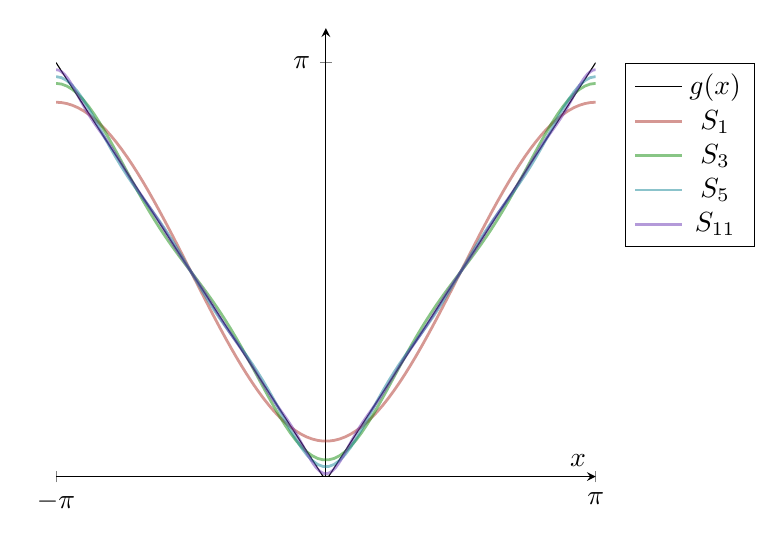
\begin{tikzpicture}
    \begin{axis}[
      axis lines = middle,
      ymax = 3.4,
      xlabel = $x$,
      ytick distance=pi,
      xtick distance=pi,
      yticklabels={,,$\pi$},
      xticklabels={,$-\pi$,,$\pi$},
      legend style={at={(axis cs:5,pi)},anchor=north east}
    ]

    \addplot[
      domain=-pi:pi,
      samples=100
    ]{
      abs(x)
    };
    \addlegendentry{$g(x)$}

    \addplot[
      domain=-pi:pi,
      samples=100,
      color={rgb,255:red,173;green,49;blue,40},
      opacity=0.5,
      line width=1pt
    ]{
      (pi/2) - cos(deg(x))*(4/pi)
    };
    \addlegendentry{$S_1$}

    \addplot[
      domain=-pi:pi,
      samples=100,
      color={rgb,255:red,19;green,140;blue,13},
      opacity=0.5,
      line width=1pt
    ]{
      (pi/2) - cos(deg(x))*(4/pi) - cos(deg(3*x))*(4/(pi*9))
    };
    \addlegendentry{$S_3$}

    \addplot[
      domain=-pi:pi,
      samples=100,
      color={rgb,255:red,24;green,136;blue,153},
      opacity=0.5,
      line width=1pt
    ]{
      (pi/2) - cos(deg(x))*(4/pi) - cos(deg(3*x))*(4/(pi*9)) 
      - cos(deg(5*x))*(4/(pi*25))
    };
    \addlegendentry{$S_5$}

    \addplot[
      domain=-pi:pi,
      samples=200,
      color={rgb,255:red,107;green,54;blue,181},
      opacity=0.5,
      line width=1pt
    ]{
      (pi/2) - cos(deg(x))*(4/pi) - cos(deg(3*x))*(4/(pi*9)) 
      - cos(deg(5*x))*(4/(pi*25)) 
      - cos(deg(7*x))*(4/(pi*49)) 
      - cos(deg(9*x))*(4/(pi*81)) 
      - cos(deg(11*x))*(4/(pi*121)) 
    };
    \addlegendentry{$S_{11}$}
      
    \end{axis}
  \end{tikzpicture}
  \caption{Graphing $g(x) = \abs{x}$, with some partial sums of the Fourier Series}
  \label{chap8:fig:fourier_absolute}
\end{figure}

The differentiated series is
\begin{equation*}
  \dv{g(x)}{x} = 
  \frac{4}{\pi}\sum_{n=1}^\infty \frac{1}{2n-1}\sin((2n-1)x),
  = f(x)
\end{equation*}
which we recognize as the Fourier Series for our step 
function from the earlier example in the text.
We cannot use the Weierstrass M-Test to conclude convergence 
for this function, as we only have $\leq K/n$ conditions,
which does not converge absolutely.

If we differentiate this series again, we get 
\begin{equation*}
  \dv{f(x)}{x} = 
  \frac{4}{\pi}\sum_{n=1}^\infty \cos((2n-1)x),
\end{equation*}
which does not converge in general.

The official solutions has a good discussion about how 
power series were more readily manipulate-able, since 
we could differentiate a power series and get another power series 
with good properties. But here, we can differentiate a continuous 
series and get a series that converges to a non-continuous function.
Not only that, but the series could even go from converging to 
not converging in general.
}
}

\bx{
$h$ is continuous over a compact set, so it is uniformly 
continuous on it too.
}

\bx{
The idea here is that since we are choosing intervals small enough
where $\sin$ completes an entire period and $\sin$ is sum-zero 
throughout this period, and we also know that $h(x)$ does not 
change a whole lot through this interval, so $h(x)$ is almost
constant so that its integral through this interval is small.

\begin{figure}[H]
  \centering
  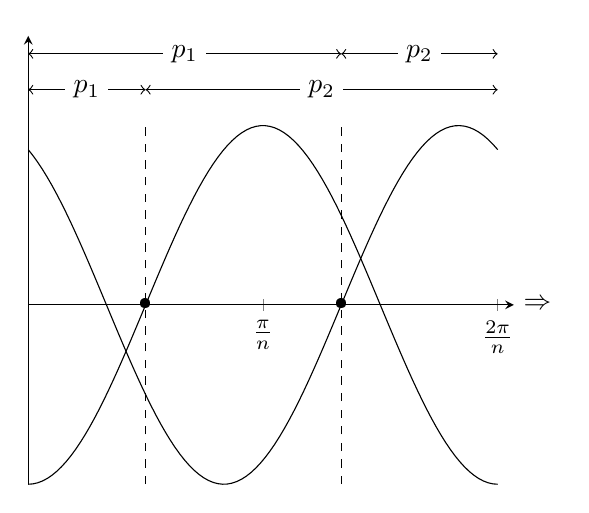
\begin{tikzpicture}
  \begin{axis}[
    axis y line = left,
    axis x line = middle,
    ymax = 1.5,
    xmax = 6.5,
    xtick distance=pi,
    ymajorticks=false,
    yticklabels = {,,},
    xticklabels = {,0,$\frac{\pi}{n}$,$\frac{2\pi}{n}$,},
    clip = false,
    x post scale=0.9
  ]

    \addplot[
      domain = 0:2*pi,
      samples=100
    ]{
      sin(deg(x-pi/2))
    };

    \addplot[
      domain = 0:2*pi,
      samples=100
    ]{
      sin(deg(x-4*pi/3))
    };

    \draw[<->]
      (axis cs:0, 1.2) --
      (axis cs:pi/2, 1.2) 
      node[midway] {\colorbox{white}{$p_1$}}
    ;

    \draw[<->]
      (axis cs:pi/2, 1.2) -- 
      (axis cs:2*pi, 1.2) 
      node[midway] {\colorbox{white}{$p_2$}}
    ;

    \draw[dashed]
      (axis cs:pi/2, -1) --
      (axis cs:pi/2, 1)
      (axis cs:pi/2, 0) node {\textbullet}
    ;

    \draw[<->]
      (axis cs:0, 1.4) --
      (axis cs:4*pi/3, 1.4) 
      node[midway] {\colorbox{white}{$p_1$}}
    ;

    \draw[<->]
      (axis cs:4*pi/3, 1.4) -- 
      (axis cs:2*pi, 1.4) 
      node[midway] {\colorbox{white}{$p_2$}}
    ;

    \draw[dashed]
      (axis cs:4*pi/3, -1) --
      (axis cs:4*pi/3, 1)
      (axis cs:4*pi/3, 0) node {\textbullet}
    ;

    \draw
      (axis cs:6.5, 0) node[right] {$\Rightarrow$}
    ;
  \end{axis}
  \end{tikzpicture}
  \begin{tikzpicture}
  \begin{axis}[
    axis y line = left,
    axis x line = middle,
    ymax = 1.5,
    xmax = 6.5,
    xtick distance=pi,
    ymajorticks=false,
    yticklabels = {,,},
    xticklabels = {,0,$\frac{\pi}{n}$,$\frac{2\pi}{n}$,},
    clip = false,
    x post scale=0.9
  ]
    \addplot[
      domain = 0:2*pi,
      samples=100
    ]{
      sin(deg(x))
    };

    \draw[<->]
      (axis cs:0, 1.25) -- 
      (axis cs:pi, 1.25) node[midway] {\colorbox{white}{$h_1(x)$}}
    ;

    \draw[<->]
      (axis cs:pi, 1.25) --
      (axis cs:2*pi, 1.25) 
      node[midway] {\colorbox{white}{$h_2(x)$}}
    ;
  \end{axis}
  \end{tikzpicture}
  \caption{
    Showing how piece together and then integrate $h(x)\sin(x)$ over a small interval
  }
  \label{chap8:fig:sine_integral}
\end{figure}

Since we know that $h$ is uniformly continuous on $\mathbb{R}$,
we can choose a $\delta$ so that $\abs{x - y} < \delta$ implies 
\begin{equation*}
  \abs{
    h(x) - h(y)
  } < \frac{\epsilon}{\pi}
\end{equation*}
Now we choose $n$ so that $\frac{2\pi}{n} < \delta$, so we still 
have this small changes in $h$ guarantee over this interval.

Now, consider some $\sin(nx)$ that completes an oscillation in 
$\pbra{a, a+2\pi/n}$. Notice how we can ``reorganize'' the curve 
and get an integral that is easier to deal with, see Figure 
\ref{chap8:fig:sine_integral}.
We can always piece together any complete sine wave into one
that starts at $0$ at the beginning of the interval 
$a$. Notice that the new $h$ functions are also jumbled, but
this is fine since we have uniform continuity, so any $h$ differences 
in this interval are small. Now,
\begin{align*}
  \int_{a}^{a+2\pi/n} h'(x)\sin(nx) \dd{x} 
  &= 
  \int_{a}^{a+\pi/n} h_1(x)\sin(nx) \dd{x} +
  \int_{a+\pi/n}^{a+2\pi/n} h_2(x)\sin(nx) \dd{x}\\
  &= 
  \int_{a}^{a+\pi/n} h_1(x)\sin(nx) \dd{x} +
  \int_{a}^{a+\pi/n} -h_2(x)\sin(nx) \dd{x}\\
  &\leq
  \int_{a}^{a+\pi/n} \abs{h_1(x)-h_2(x)}\abs{\sin(nx)} \dd{x}\\
  &<
  \int_{a}^{a+\pi/n} \frac{\epsilon}{\pi}\sin(nx) \dd{x}\tag{
    Uniform continuity of $h$, $\sin(nx) \geq 0$ on first half of period
  }\\
  &=
  \int_{0}^{\pi/n} \frac{\epsilon}{\pi}\sin(nx) \dd{x} 
  \tag{$\sin(nx)$ starts its period at $a$)}\\
  &\leq
  \frac{\epsilon}{\pi} \frac{\pi}{n} = \frac{\epsilon}{n}
  \tag{$\sin(x) \leq 1$}
\end{align*}
So for any integral over $\pbra{-\pi, \pi}$, 
we have $n$ of these $\sin$ complete periods, so 
\begin{equation*}
  \int_{-\pi}^\pi h(x)\sin(nx) \dd{x} < n \cdot \frac{\epsilon}{n} = \epsilon
\end{equation*}

A similar argument holds for the $\cos$ integral.
}

\bx{
\ea{
\item $q_x(u)$ is the sum of two continuous functions,
so itself is also continuous. Then by the Riemann-Lebesgue Lemma,
we know this integral tends to 0 as $N \to \infty$.

\item Our goal is to show that $p_x(u)$ is continuous so that 
we can use the Riemann-Lebesgue Lemma.

Our main roadblock is that at $u=0$, we have $\sin(u/2) = 0$,
which is a a dividing by 0 issue. However, if we can define 
a value at $0$ for $p_x$ to make it continuous, then we can still
do the integral.

Observe that 

\begin{align*}
  \lim_{u \to 0} p_x(u) 
  &= 
  \lim_{u \to 0}
  \frac{
    f(u+x) - f(x)
  }{
    u
  }
  \frac{u\cos(u/2)}{\sin(u/2)}\\
  &=
  \lim_{u \to 0}
  f'(x)
  \frac{u\cos(u/2)}{\sin(u/2)}\\
  &=
  f'(x)
  \frac{
    \lim_{u \to 0}
    \cos(u/2) - \frac{u}{2}\sin(u/2)
  }{
    \lim_{u \to 0} \cos(u/2)/2
  }\\
  &= 2 f'(x),
\end{align*}
so this limit exists, and we can assign $p_x(0) = 2 f'(x)$,
so make $p_x$ continuous.

Then by the Riemann-Lebesgue Lemma, we conclude this integral 
goes to 0.

This will complete the proof since 
\begin{equation*}
  \lim{N \to \infty} S_N(x) - f(x) \to 0
  \Rightarrow S_N(x) \to f(x)
\end{equation*}
}
}

\bx{
The idea here is that as we add more terms, the weight of the 
average shifts more towards the terms that appear a lot.
If $x_n \to L$, then at the end, all the terms are close to $L$,
so if we keep on increasing their weight, then the bias weight
favors $L$.

We can tkae $y_n = (-1)^n$,
then $\abs{y_{2n}} \leq 1/n$, so $y_n \to 0$.
But the original sequence oscillates around $-1, 0$,
so it never converges.
}

\bx{
\begin{align*}
  \frac{
    1/2 + \sum_{n=1}^N D_n(\theta)
  }{
    N+1
  }
  &=
  \frac{
    1/2 + \sum_{n=1}^N \frac{\sin((n+1/2)\theta)}{2\sin(\theta/2)}
  }{
    N+1
  }\\
  &=
  \frac{
    1/2 + \frac{1}{2\sin(\theta/2)}\sum_{n=1}^N \sin((n+1/2)\theta)
  }{
    N+1
  }\\
  &=
  \frac{
    1/2 + \frac{1}{2\sin(\theta/2)}
    \sum_{n=1}^N \pbra{
      \sin(n\theta)\cos(\theta/2) + 
      \sin(\theta/2)\cos(n\theta)
    }
  }{
    N+1
  }\tag{Sum angle}\\
  &=
  \frac{
    1
  }{
    2(N+1)
  }
  \pbra{
    \frac{1}{2}
    +
    \frac{1}{2}
    +
    \sum_{n=1}^N \cos(n\theta)
    +
    \frac{\cos(\theta/2)}{\sin(\theta/2)}
    \sum_{n=1}^N \sin(n\theta)
  }\\
  &=
  \frac{
    1
  }{
    2(N+1)
  }
  \pbra{
    \frac{1}{2}
    +
    \frac{\sin((N+1/2)\theta)}{2\sin(\theta/2)}
    +
    \frac{\cos(\theta/2)}{\sin(\theta/2)}
    \cdot
    \frac{\sin(N\theta/2)\sin((N+1)\theta/2)}{\sin(\theta/2)}
  }\\
  &=
  \frac{
    1
  }{
    2(N+1)
  }
  \pbra{
    \frac{\sin^2(\theta/2)}{2\sin^2(\theta/2)}
    +
    \frac{\sin((N+1/2)\theta)\sin(\theta/2)}{2\sin^2(\theta/2)}
    +
    \frac{2\sin(N\theta/2)\sin((N+1)\theta/2)\cos(\theta/2)}{2\sin^2(\theta/2)}
  }
\end{align*}
This is honestly just a trig computation exercise... 

An idea to simplify this is since we know the final answer,
expand out 
\begin{equation*}
  \pbra{
    \sin((N+1)\theta/2)
  }^2 = \pbra{
    \sin(N\theta/2)\cos(\theta/2) +
    \sin(\theta/2)\cos(N\theta/2)
  }
\end{equation*}
and try to match terms. 
A good approach is to first get rid of all the angle sums by
expanding them out, and cancelling what is in common.
Then, use double and half 
angle formulas to simplify the result. 
}

\bx{
\ea{
\item A lot of calculation. Some of this can be used from ealier when we 
proved the Riemann-Lebesgue lemma.
\begin{align*}
  \sigma_N(x) 
  &=
  \frac{1}{N+1}\sum_{n=0}^N S_N(x)\\
  &=
  \frac{1}{N+1}\sum_{n=0}^N \pbra{
    a_0 + \sum_{m=1}^n a_n\cos(nx) + b_n\sin(nx)
  }\\
  &=
  \frac{1}{N+1}\sum_{n=0}^N \pbra{
    \frac{1}{2\pi}\int_{-\pi}^\pi f(t) \dd{t}
    + 
    \frac{1}{\pi}
    \sum_{m=1}^n \int_{-\pi}^\pi \pbra{
      f(t)\cos(nt)\cos(nx) + f(t)\sin(nt)\sin(nx)
    } \dd{t}
  }\\
  &=
  \frac{1}{N+1}\sum_{n=0}^N \pbra{
    \frac{1}{\pi}
    \int_{-\pi}^\pi
    f(t) \pbra{
      \frac{1}{2} + 
      \sum_{m=1}^n 
      \cos(n(t-x))
    }
    \dd{t}
  }\\
  &=
  \frac{1}{N+1}\sum_{n=0}^N \pbra{
    \frac{1}{\pi}
    \int_{-\pi}^\pi
    f(t) D_n(t-x)
    \dd{t}
  }\\
  &=
  \frac{1}{N+1}
  \frac{1}{\pi}
  \int_{-\pi}^\pi
  f(t) \pbra{
    \sum_{n=0}^N
    D_n(t-x)
  } \dd{t}\\
  &=
  \frac{1}{\pi}
  \int_{-\pi}^\pi
  f(t) \frac{1}{N+1}\pbra{
    1/2 +
    \sum_{n=1}^N
    D_n(t-x)
  } \dd{t}
  \tag{When $n=0$, there are no $\cos$ terms}\\
  &=
  \frac{1}{\pi}
  \int_{-\pi}^\pi
  f(t) F_N(t-x)
  \dd{t}\tag{Fej\'{e}r kernel}\\
  &=
  \frac{1}{\pi}
  \int_{-\pi-x}^{\pi-x}
  f(u+x) F_N(u)
  \dd{u}\tag{$u=t-x$}\\
  &=
  \frac{1}{\pi}
  \int_{-\pi}^{\pi}
  f(u+x) F_N(u)
  \dd{u}\tag{$f$ periodic over $2\pi$}\\
\end{align*}

\item Graphing $F_N(u)$,
\begin{figure}[H]
  \centering
  \subfloat[Graphing $F_N(x)$ for different values of $N$]{
  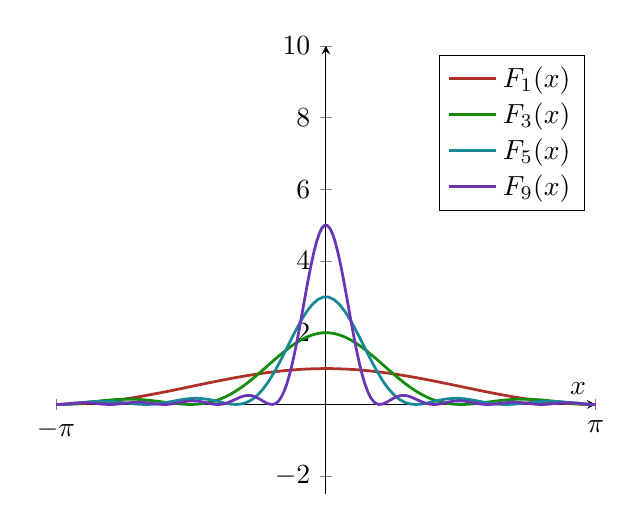
\begin{tikzpicture}
  \begin{axis}[
    axis lines = middle,
    ymax = 10,
    ymin = -2.5,
    xtick distance=pi,
    xticklabels={,$-\pi$,,$\pi$,},
    xlabel = $x$,
    every axis plot/.append style={line width=1pt}
  ]
    \def\nval{1}
    \addplot[
      domain=-pi:pi,
      samples=100,
      color={rgb,255:red,173;green,49;blue,40}
    ]{
      (1/(2*(\nval+1)))*(
        sin(deg((\nval+1)*x/2))/
        sin(deg(x/2))
      )^2
    };
    \addlegendentry{$F_{1}(x)$}

    \def\nval{3}
    \addplot[
      domain=-pi:pi,
      samples=100,
      color={rgb,255:red,19;green,140;blue,13}
    ]{
      (1/(2*(\nval+1)))*(
        sin(deg((\nval+1)*x/2))/
        sin(deg(x/2))
      )^2
    };
    \addlegendentry{$F_{3}(x)$}

    \def\nval{5}
    \addplot[
      domain=-pi:pi,
      samples=100,
      color={rgb,255:red,24;green,136;blue,153}
    ]{
      (1/(2*(\nval+1)))*(
        sin(deg((\nval+1)*x/2))/
        sin(deg(x/2))
      )^2
    };
    \addlegendentry{$F_{5}(x)$}

    \def\nval{9}
    \addplot[
      domain=-pi:pi,
      samples=200,
      color={rgb,255:red,107;green,54;blue,181}
    ]{
      (1/(2*(\nval+1)))*(
        sin(deg((\nval+1)*x/2))/
        sin(deg(x/2))
      )^2
    };
    \addlegendentry{$F_{9}(x)$}
  \end{axis}
  \end{tikzpicture}
  }
  \subfloat[Graphing $D_N(x)$]{
  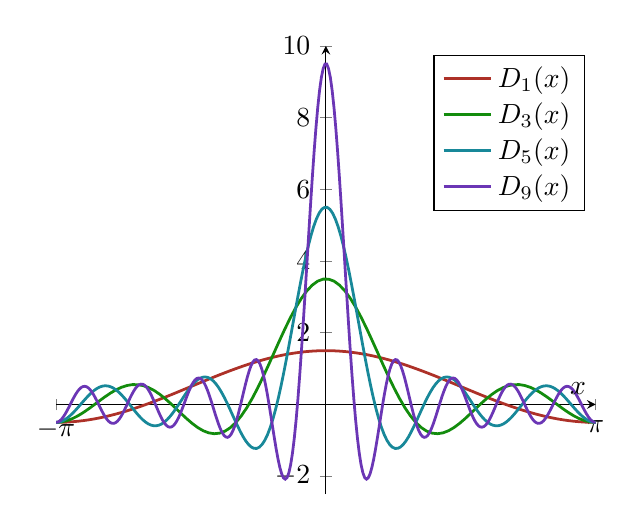
\begin{tikzpicture}
  \begin{axis}[
    axis lines = middle,
    ymax = 10,
    ymin = -2.5,
    xtick distance=pi,
    xticklabels={,$-\pi$,,$\pi$,},
    xlabel = $x$,
    every axis plot/.append style={line width=1pt}
  ]
    \def\nval{1}
    \addplot[
      domain=-pi:pi,
      samples=100,
      color={rgb,255:red,173;green,49;blue,40}
    ]{
      sin(deg(
        x*(\nval+1/2)
      ))/(
        2*sin(deg(x/2))
      )
    };
    \addlegendentry{$D_{1}(x)$}

    \def\nval{3}
    \addplot[
      domain=-pi:pi,
      samples=100,
      color={rgb,255:red,19;green,140;blue,13}
    ]{
      sin(deg(
        x*(\nval+1/2)
      ))/(
        2*sin(deg(x/2))
      )
    };
    \addlegendentry{$D_{3}(x)$}

    \def\nval{5}
    \addplot[
      domain=-pi:pi,
      samples=200,
      color={rgb,255:red,24;green,136;blue,153}
    ]{
      sin(deg(
        x*(\nval+1/2)
      ))/(
        2*sin(deg(x/2))
      )
    };
    \addlegendentry{$D_{5}(x)$}

    \def\nval{9}
    \addplot[
      domain=-pi:pi,
      samples=300,
      color={rgb,255:red,107;green,54;blue,181}
    ]{
      sin(deg(
        x*(\nval+1/2)
      ))/(
        2*sin(deg(x/2))
      )
    };
    \addlegendentry{$D_{9}(x)$}
  \end{axis}
  \end{tikzpicture}
  }
  \caption{Comparing $F_N, D_N$.}
  \label{chap8:fig:fejer_kernel}
\end{figure}
We see that $F_N(x)$ is larger at $x = 0$, which makes sense 
since we have $\sin^2(\theta/2)$ in the denominator.
Everywhere else, $F_N(x)$ is small.

Compared with $D_N(x)$, $F_N(x)$ has a smaller magnitude at $0$,
and also is all positive.

If we want to show $F_n \to 0$, intuitively, as $N \to \infty$,
it seems that the middle peak gets more narrow, although higher,
and the width becomes closer and closer to 0.

Formally, we essentially need to show that 
for $\abs{\theta} \geq \delta$, $\exists N, \abs{F_N} < \epsilon$.

First, we fix $\theta > 0$.
The challenge here is that we don't know how big 
our expression can be, but our goal is to show 
it is finite, but also able to be diminished by $\frac{1}{N}$,
\begin{align*}
  \abs{
    F_N(\theta)
  } &=
  \abs{
    \frac{
      1
    }{2(N+1)}
    \pbra{
      \frac{
        \sin((N+1)\theta/2)
      }{
        \sin(\theta/2)
      }
    }^2
  }\\
  &=
  \frac{
    1
  }{2(N+1)}
  \abs{
    \pbra{
      \frac{
        \sin(N\theta/2)\cos(\theta/2) + \sin(\theta/2)\cos(N\theta/2)
      }{
        \sin(\theta/2)
      }
    }^2
  }\\
  &=
  \frac{
    1
  }{2(N+1)}
  \abs{
    \pbra{
      \sin(N\theta/2)\frac{\cos(\theta/2)}{\sin(\theta/2)} + 
      \cos(N\theta/2)
    }^2
  }\\
  &=
  \frac{
    1
  }{2(N+1)}
  \abs{
    \sin^2(N\theta/2)\frac{\cos^2(\theta/2)}{\sin^2(\theta/2)} + 
    2\sin(N\theta/2)\cos(N\theta/2)\frac{\cos(\theta/2)}{\sin(\theta/2)} + 
    \cos^2(N\theta/2)
  }
\end{align*}
Here, since $\theta$ is fixed, we can say
\begin{equation*}
  \frac{
    \cos(\theta/2)
  }{
    \sin(\theta/2)
  } = K
\end{equation*}

That means we can write
\begin{equation*}
  \lim_{N\to\infty}
  \frac{
    1
  }{2(N+1)}
  \abs{
    \sin^2(N\theta/2)\frac{\cos^2(\theta/2)}{\sin^2(\theta/2)} + 
    2\sin(N\theta/2)\cos(N\theta/2)\frac{\cos(\theta/2)}{\sin(\theta/2)} + 
    \cos^2(N\theta/2)
  }
  \leq
  \lim_{N\to\infty}
  \frac{
    1
  }{2(N+1)}
  \abs{
    K^2 + 
    2K +
    1
  } = \epsilon
\end{equation*}

\item We can see that 
\begin{align*}
  \int_{-\pi}^\pi F_N(u) \dd{u}
  &=
  \int_{-\pi}^\pi
  \frac{
    1/2 + \sum_{n=1}^N D_n(u)
  }{
    N+1
  }
  \dd{u}\\
  &=
  \frac{ 1 }{ N+1 }
  \int_{-\pi}^\pi
    1/2 + \sum_{n=1}^N D_n(u)
  \dd{u}\\
  &=
  \frac{ 1 }{ N+1 }\pbra{
    \pi + 
    \sum_{n=1}^N \int_{-\pi}^\pi D_n(u) \dd{u}
  }\\
  &=
  \frac{ 1 }{ N+1 }\pbra{
    \pi + 
    \sum_{n=1}^N \pi
  }\\
  &= \frac{1}{N+1} \cdot (N+1)\pi = \pi
\end{align*}

\item We can first set up our integral,
\footnote{the text has a typo here, asking for $\sigma_Nf(x) - f(x)$}
\begin{align*}
  \sigma_N(x) - f(x) 
  &= 
  \frac{1}{\pi}
  \int_{-\pi}^\pi 
  \pbra{
    f(u+x)F_N(u) \dd{u}
  } - f(x) \cdot \frac{1}{\pi}\int_{-\pi}^\pi F_N(u) \dd{u}\\
  &=
  \frac{1}{\pi}
  \int_{-\pi}^\pi 
    \pa{f(u+x) - f(x)}F_N(u) \dd{u}
\end{align*}
}
Now, we split our integral,
\begin{align*}
  \frac{1}{\pi}
  \int_{-\pi}^\pi 
    \pa{f(u+x) - f(x)}F_N(u) \dd{u}
  &= \int_{\abs{u} < \delta}
    \pa{f(u+x) - f(x)}F_N(u) \dd{u} +
  \int_{\abs{u} \geq \delta}
    \pa{f(u+x) - f(x)}F_N(u) \dd{u}
\end{align*}
We can bound the $\abs{u} < \delta$ integral by
choosing $\delta$ small enough so that for $\abs{x - y} < \delta$,
$\abs{f(x) - f(y)} < \epsilon/(2\pi)$.
\footnote{
  We can do this because we showed $f$ to be uniformly continuous.
}
Then we can show,
\begin{align*}
  \int_{\abs{u} < \delta}
    \abs{f(u+x) - f(x)}F_N(u) \dd{u}
  &\leq \int_{-\pi}^\pi
    \frac{\epsilon}{2\pi} F_N(u) \dd{u}\tag{Including more}\\
  &\leq 
  \frac{\epsilon}{2}
\end{align*}
For the $\abs{u} \geq \delta$ integral, 
first choose $N$ so that $F_N(u) < \frac{\epsilon}{8M\pi}$\footnote{
As a reminder, we can do this because $F_N(u) \to 0$ for $\abs{u} > 0$.
},
where $M$ is the bound of $f$, then 
\begin{align*}
  \int_{\abs{u} \geq \delta}
    \pa{f(u+x) - f(x)}F_N(u) \dd{u}
  &\leq
  \int_{\abs{u} \geq \delta}
    2M F_N(u) \dd{u}\\
  &<
  \int_{\abs{u} \geq \delta}
    2M \cdot \frac{\epsilon}{8M\pi} \dd{u}\\
  &\leq
  \int_{-\pi}^\pi
    \frac{\epsilon}{4\pi} \dd{u}\\
  &=
  2\pi \cdot \frac{\epsilon}{4\pi} = \frac{\epsilon}{2}
\end{align*}
so together, we have the two integrals add up to $< \epsilon$,
and therefore we can conclude 
\begin{equation*}
  \sigma_N(x) \to f(x)
\end{equation*}
}

\bx{
\ea{
\item We want to use $\sigma_N(x)$ as the sequence of functions 
that converges to $f(x)$ uniformly. The only issue is that $\sigma_N(x)$
is a partial sum of $\sin, \cos$, which are infinite series 
and therefore not polynomials.

However, we can always find polynomials that are arbitrarily 
close to $\sin, \cos$, so we can always 
construct such polynomials that converge to $f(x)$ uniformly,
using $\sigma_N(x)$ as a reference.

\item Once we have proved it works for a certain interval,
we can always just translate the function into $[0, \pi]$,
show it is true, and then translate it back.
}
}